\documentclass{extarticle}
\usepackage{arxiv}
\usepackage[utf8]{inputenc}
\usepackage[X2, T2A]{fontenc}
\usepackage[english, russian]{babel}
\usepackage{graphicx}
\usepackage{amsmath, amssymb, amsthm}
\usepackage{indentfirst}
\usepackage{listings}
\usepackage{upquote}
\usepackage{hyperref}
\usepackage{xcolor}
\usepackage{mathtools}
\usepackage{float}
\sloppy

% старые символы кириллицы
\DeclareTextSymbolDefault{\CYRYAT}{X2}
\DeclareTextSymbolDefault{\cyryat}{X2}

\makeatletter
%   from Report.sty:
%   Create caption "Fig. 1." instead of "Fig. 1:"
\long\def\@makecaption#1#2{%
	\vskip 10\p@
	\setbox\@tempboxa\hbox{#1. #2}%
	\ifdim \wd\@tempboxa >\hsize
	#1. #2\par
	\else
	\hbox to\hsize{\hfil\box\@tempboxa\hfil}%
	\fi}
\makeatother


\title{Распознавание рукописных архивов А. В. Сухово-Кобылина}

\author{ Зыков Валерий Павлович \\
	ВМК МГУ\\
	\texttt{zykovvp@my.msu.ru} \\
	%% examples of more authors
	\And
	Местецкий Леонид Моисеевич \\
	ВМК МГУ \\
	\texttt{mestlm@mail.ru} \\
}
\date{2024}


\begin{document}
\maketitle
\begin{abstract}
	В данной работе решается задача распознавания рукописных архивов А. В. Сухово-Кобылина, важного исторического источника XIX века. Задача осложняется плотной компоновкой строк, многоязычностью и неполной разметкой текста. Для её решения применяется подход, основанный на модели Vertical Attention Network (VAN), адаптированной под особенности данного архива. Новизна работы заключается в адаптации модели к рукописям с характерными историческими и лингвистическими особенностями. Представлены результаты экспериментов по обучению модели на данных архива и рассмотрены перспективы дальнейшего улучшения качества распознавания.
\end{abstract}

\keywords{Распознавание текста, Рукописные архивы, Vertical Attention Network, Исторические документы, Сегментация строк, Исправление текста, Машинное обучение, ChatGPT}



\section{Введение}

Распознавание рукописных исторических архивов — сложная задача, требующая адаптации современных методов компьютерного зрения и обработки текста к уникальным особенностям рукописей. Архивы А. В. Сухово-Кобылина, важного исторического источника XIX века, содержат тысячи страниц с плотным текстом, различными стилями письма и языковыми вставками, что значительно усложняет задачу их расшифровки.

\textbf{Цель исследования} — разработка метода распознавания рукописных текстов, который эффективно работает с архивами Сухово-Кобылина. В отличие от классических End-to-End подходов, которые пытаются распознать текст на уровне всей страницы, в данной работе используется метод сегментации строк с последующим их распознаванием строчной моделью. Этот подход позволяет более эффективно обрабатывать рукописи с нерегулярной структурой текста.

\textbf{Основные термины}. Распознавание рукописей подразумевает автоматическое преобразование изображения рукописного текста в машиночитаемый формат. В данном случае, сегментация строк выполняется на предварительном этапе, после чего каждая строка обрабатывается отдельно с использованием строчной модели. Vertical Attention Network (VAN) — модель, использующая механизм вертикального внимания для распознавания строк текста, что делает её подходящей для обработки рукописей с нелинейными строками.

\textbf{Проблема}. Сложность задачи распознавания рукописей обусловлена не только различиями в почерке, но и низким качеством изображений, наличием пропусков и зачеркиваний, а также многоязычной разметкой. Текущие работы по распознаванию архивов Литке \cite{peter_dataset, stepochkin} и русскоязычных рукописных текстов \cite{yandex} показывают, что классические модели, такие как CRNN, часто не справляются с такими сложностями.

\textbf{Современные решения}. Недавно предложены новые архитектуры для распознавания рукописных текстов: SPAN \cite{SPAN}, TrOCR \cite{TrOCR}, и Vertical Attention Network (VAN) \cite{VAN}. SPAN и TrOCR обеспечивают высокую точность на страницах с линейными строками, однако их применение ограничено при работе с архивами, где текст организован нерегулярно. Строчная модель VAN была выбрана для работы с архивами Сухово-Кобылина, так как она позволяет эффективно распознавать строки текста с учетом их нелинейности и многоязычной структуры.

\textbf{Методология}. В данной работе используется модифицированная версия строчной модели VAN, адаптированная для архивов Сухово-Кобылина. Процесс сегментации на строки выполнялся программой, разработанной Л. М. Местецким, а для пост-обработки текста использовалась языковая модель GPT с few-shot learning для исправления ошибок в распознавании.

\textbf{Новизна}. Предлагаемый подход использует механизм вертикального внимания для распознавания рукописей с плотной компоновкой текста и многоязычными вставками. Преимущество этого метода заключается в отказе от End-to-End распознавания всей страницы и переходе к распознаванию отдельных строк, что позволяет более эффективно работать с документами, где строки нелинейны или расположены неравномерно.

Эксперименты проводились на наборе данных, включающем 92 страницы дневников Сухово-Кобылина ($\approx 1700$ строк). Для повышения точности модель была предварительно обучена на датасете IAM и дообучена с использованием CTC-loss на архиве Сухово-Кобылина с учётом пропусков символов.


\section{Постановка задачи}

Основной задачей является автоматизация процесса распознавания рукописных страниц архивов А. В. Сухово-Кобылина. Объектом исследования выступает архив, содержащий более 10 000 неразмеченных страниц и 92 размеченные страницы с текстом, записанным на русском языке XIX веке.

\textbf{Набор данных}. Для обучения используется набор данных, состоящий из изображений страниц с размеченными строками. Пример исходной рукописной страницы изображен на рис. \ref{fig:example_page}. В процессе разметки были учтены особенности текста, такие как многоязычные вставки (русский и французский языки), плотная компоновка строк, а также наличие зачеркиваний и пропусков символов. Для обучения используется метод предобучения на схожих данных, таких как IAM, с последующим дообучением на разметке архива Сухово-Кобылина. Данные имеют следующие особенности:
\begin{itemize}
	\item Многоязычные вставки (русский и французский языки).
	\item Плотная компоновка строк и нерегулярные зачеркивания.
	\item Пропуски символов и неразборчивые фрагменты текста.
\end{itemize}

\begin{figure}[h!]
	\centering
	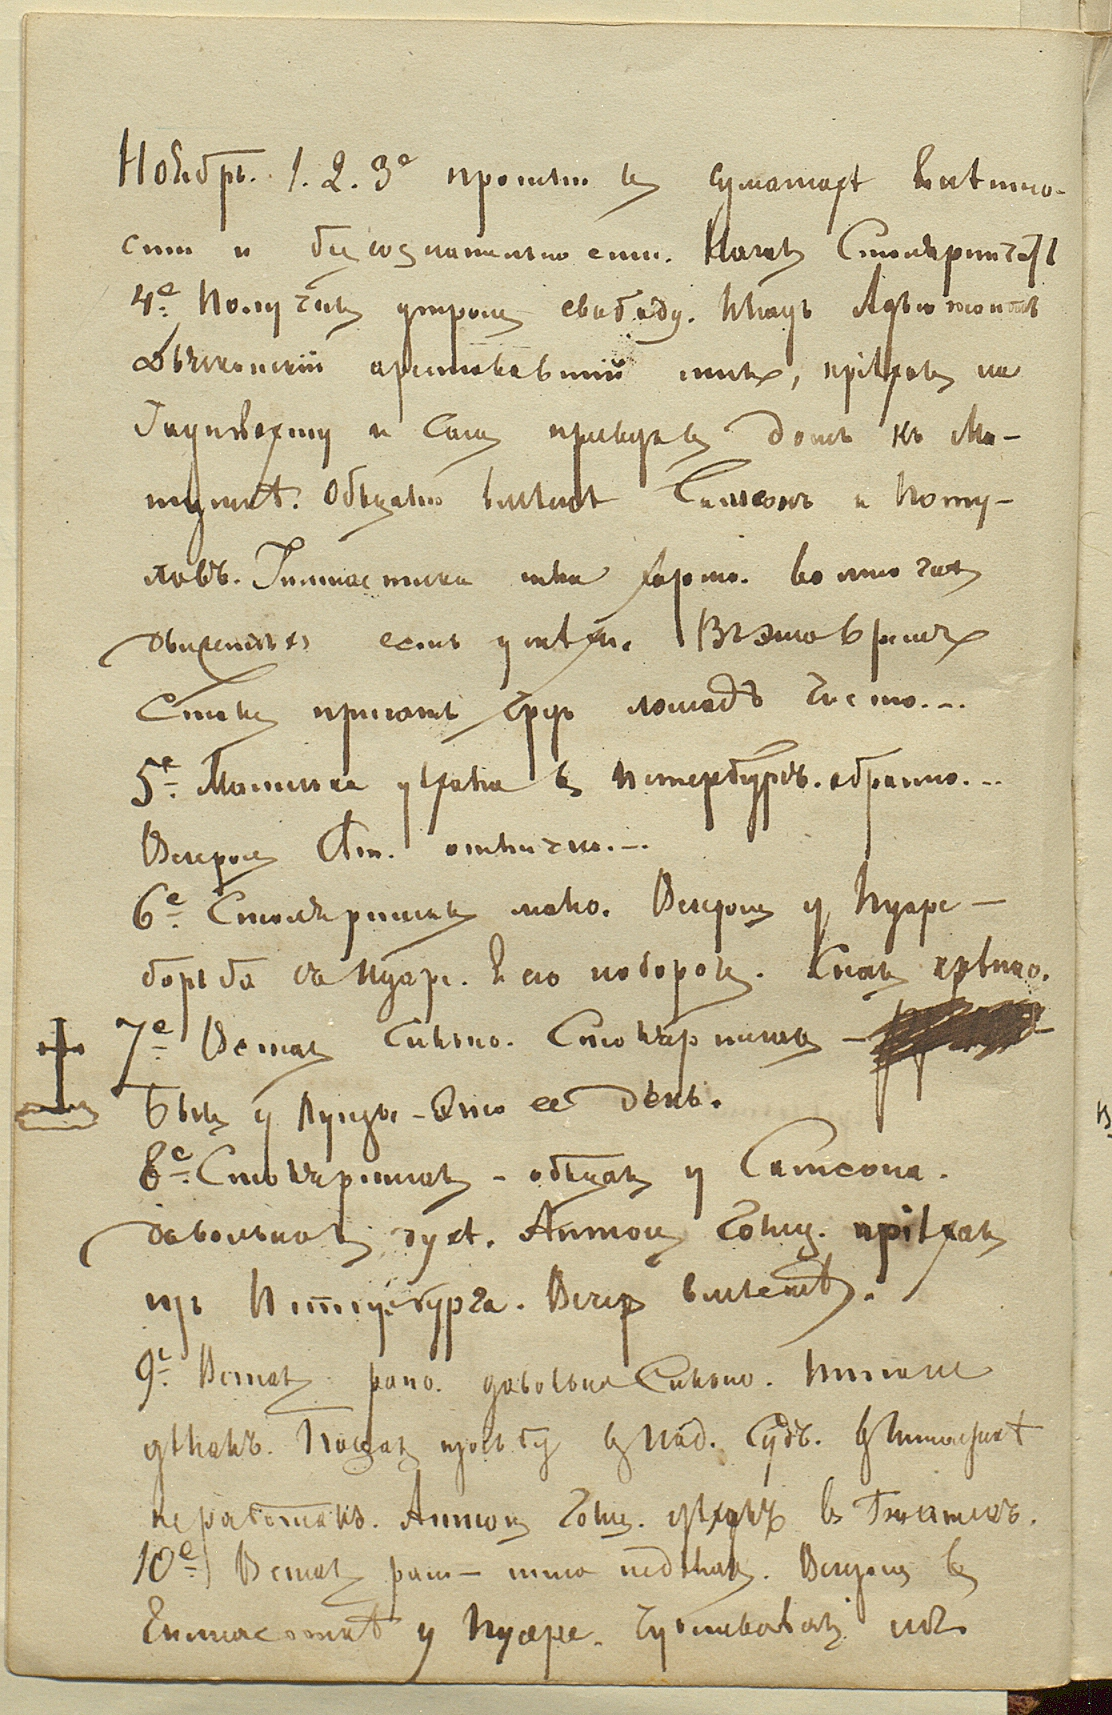
\includegraphics[width=0.6\textwidth]{images/пример.jpg}
	\caption{Пример исходной страницы дневника А. В. Сухово-Кобылина}
	\label{fig:example_page}
\end{figure}

\textbf{Метод}. Для решения задачи используется модель \textit{Vertical Attention Network} (VAN) в строчной модификации, способная распознавать текст на уровне строк. Это параметрическое семейство функций, преобразующих изображение в последовательность символов, используя сверточные слои и механизм вертикального внимания. Модель обучается с использованием функции потерь CTC-loss, которая подходит для работы с последовательностями символов, допускающими пропуски.

\textbf{Критерии качества}. Для оценки работы модели используются метрики CER (Character Error Rate) и WER (Word Error Rate), которые измеряют количество ошибок на уровне символов и слов соответственно. Эти метрики отслеживаются как на тренировочной, так и на валидационной выборках для выбора наилучшего чекпоинта модели.

\textbf{Целевая функция} минимизирует CTC-loss, оптимизируя параметры модели:
\[
\hat{\theta} = \arg\min_\theta \mathcal{L}_{CTC}(y, \hat{y}(\theta)),
\]
где \(y\) — правильная последовательность символов, \(\hat{y}(\theta)\) — предсказанная последовательность модели с параметрами \(\theta\).

\textbf{Процедура обучения}. Обучение проводится в два этапа: сначала происходит предобучение модели на датасете IAM, затем проводится дообучение на разметке архива Сухово-Кобылина. Набор данных для обучения состоит из 1505 строк для тренировки, 119 строк для валидации и 74 строки для тестирования. В процессе обучения используется стратегия отслеживания метрик на валидационной выборке для выбора наилучшего чекпоинта.

\textbf{Ограничения и предположения}. В процессе обучения предполагается, что данные могут содержать ошибки разметки, такие как неразборчивые фрагменты текста или пропуски символов. Кроме того, учитывается, что строки в архиве Сухово-Кобылина могут быть нелинейными и имеют сложную структуру, что требует применения метода сегментации строк перед распознаванием. Эти ограничения учитываются при выборе архитектуры модели и стратегии обучения.



\section{Вычислительный эксперимент}

Цель базового эксперимента заключается в обучении строчной модели Vertical Attention Network (VAN) на двух датасетах: READ\_2016 и IAM. Задача заключалась в получении базовых метрик для этих данных с минимальными усилиями, что позволило бы оценить производительность модели и её способность к обучению на различных наборах рукописных данных.

\subsection{Базовый набор данных}

Для эксперимента использовались два публичных датасета:

\begin{itemize}
	\item \textbf{READ\_2016}: Содержит набор данных для распознавания рукописных текстов на немецком языке раннего Нового времени. Датасет состоит из различных рукописных фрагментов, включая тексты с зачеркиваниями и сложными почерками.
	\item \textbf{IAM}: Содержит англоязычные рукописные данные для распознавания текстов, включая как письменные заметки, так и формализованные тексты. Этот датасет является стандартом для задач распознавания рукописных текстов.
\end{itemize}

\textbf{Условия проведения измерений}: На каждом датасете был проведен процесс обучения модели на тренировочной части данных, затем модель была проверена на валидационной и тестовой частях. Все эксперименты проводились на одном и том же оборудовании.

\textbf{Статистика}: 
\begin{itemize}
	\item \textbf{READ\_2016}: Тренировочная часть — 8349 строк, валидационная — 1040 строк, тестовая — 1138 строк.
	\item \textbf{IAM}: Тренировочная часть — 6482 строк, валидационная — 976 строка, тестовая — 2915 строк.
\end{itemize}

\subsection{Конфигурация эксперимента}

Модель обучалась с использованием функции потерь CTC-loss. В качестве кодировщика использовалась строчная версия Vertical Attention Network (VAN). 

\subsection{Результаты на датасете READ\_2016}

Модель была обучена на датасете READ\_2016 в течение 130 эпох. Результаты на различных частях датасета следующие:

\begin{itemize}
	\item \textbf{Тренировочная часть}: CER = 4.36\%, WER = 17.92\%
	\item \textbf{Валидационная часть}: CER = 7.14\%, WER = 27.76\%
	\item \textbf{Тестовая часть}: CER = 7.01\%, WER = 26.54\%
\end{itemize}

\subsection{Результаты на датасете IAM}

Модель была обучена на датасете IAM в течение 1832 эпох. Результаты на различных частях датасета следующие:

\begin{itemize}
	\item \textbf{Тренировочная часть}: CER = 0.35\%, WER = 1.40\%
	\item \textbf{Валидационная часть}: CER = 3.88\%, WER = 13.29\%
	\item \textbf{Тестовая часть}: CER = 5.58\%, WER = 18.11\%
\end{itemize}

\subsection{Заключение по базовому эксперименту}

Результаты базового эксперимента показали, что модель VAN с функцией потерь CTC-loss может эффективно обучаться на различных датасетах рукописных текстов. На датасете IAM модель показала хорошие результаты, что свидетельствует о высокой точности распознавания для английского языка. На датасете READ\_2016 результаты были несколько хуже, что обусловлено тем, что модель на этом датасете обучалась сильно меньше эпох по сравнению с датасетом IAM.

Эти результаты послужили основой для дальнейшего обучения модели на данных архива Сухово-Кобылина, где была проведена инициализация весов кодировщика на основе модели, обученной на IAM.

\section{Теоретическая часть}

\subsection{Архитектура модели VAN}

Для решения задачи распознавания рукописных архивов была выбрана модель Vertical Attention Network (VAN), которая показала высокую эффективность в задачах распознавания рукописных документов \cite{VAN}. Архитектура VAN позволяет использовать механизмы вертикального внимания для анализа текстовых страниц, автоматически выделяя строки и распознавая их содержимое. Существуют два основных варианта модели: страничная и строчная.

\subsubsection{Страничная архитектура}

Страничная модель VAN разработана для распознавания текста на уровне всей страницы без необходимости сегментации на строки. Она предполагает, что строки текста являются линейными и ровными, что упрощает процесс их распознавания, но делает модель менее гибкой при обработке рукописей с нелинейными строками. Кодировщик страницы состоит из сверточных слоев, которые извлекают пространственные признаки, после чего механизм вертикального внимания рекурсивно определяет строки текста, разделяя изображение на строки для дальнейшего распознавания.

\begin{figure}[H]
	\centering
	\includegraphics[width=0.99\textwidth]{images/архитектура_страничная.pdf}
	\caption{Страничная архитектура VAN}
	\label{fig:page_architecture}
\end{figure}

\subsubsection{Строчная архитектура}

Для нашей задачи была выбрана строчная версия модели VAN, которая работает с отдельными строками текста. Этот подход более подходящий для распознавания архивов Сухово-Кобылина, так как структура данных сложная, строки могут быть нелинейными, а также имеется ограниченное количество данных для обучения. В строчной архитектуре текст сегментируется на строки, которые затем подаются на вход модели. Основная задача кодировщика заключается в преобразовании изображения строки в набор признаков, которые обрабатываются далее декодировщиком для предсказания символов.

\begin{figure}[H]
	\centering
	\includegraphics[width=0.99\textwidth]{images/архитектура_строчная.pdf}
	\caption{Строчная архитектура VAN}
	\label{fig:line_architecture}
\end{figure}

\subsubsection{Кодировщик}

Кодировщик в обеих версиях модели (строчной и страничной) одинаков и состоит из сверточных слоев, которые извлекают пространственные признаки изображения. Эти признаки затем передаются декодировщику, который производит распознавание текста на уровне символов.

\begin{figure}[H]
	\centering
	\includegraphics[width=0.99\textwidth]{images/кодировщик.pdf}
	\caption{Кодировщик VAN (одинаковый для страничной и строчной архитектур)}
	\label{fig:encoder}
\end{figure}

\subsection{Процедура нарезки страницы на строки}

Для строчной модели необходимо сначала сегментировать изображение страницы на отдельные строки. Эта процедура была выполнена с помощью программы, разработанной Л. М. Местецким. Алгоритм сегментации включает несколько шагов:

\begin{enumerate}
	\item Изображение страницы переводится в полутоновое (серое) изображение.
	\item Для каждой строки изображения вычисляется сумма яркостей пикселей по столбцам. Получаем функцию, зависящую от ординаты. Эта функция имеет форму синусоиды, минимумы которой соответствуют позициям строк.
	\item Страницу можно разделить на вертикальные сегменты, и для каждого сегмента выполнить данную операцию, чтобы учесть нелинейность строк. Мы разбивали страницу на 2 сегмента.
	\item Полученные базовые линии строк на разных сегментах объединяются в виде двухзвенных ломаных линий, описывающих положение строк на изображении.
	\item Далее от базовых линий отступают на некоторое количество пикселей вверх и вниз, чтобы выделить ограничивающие прямоугольники для каждой строки.
	\item После этого выполняется нормализация строк — двухзвенные ломаные линии выпрямляются с помощью сдвига значений в столбцах изображения, получая выпрямленные строки для подачи в строчную модель.
\end{enumerate}

\subsubsection{Пример выделения линий строк}

На рисунке \ref{fig:line_detection_1_2} показан пример исходного изображения страницы и результат выделения базовых линий строк с использованием программы.

\begin{figure}[H]
	\centering
	\begin{minipage}{0.49\textwidth}
		\centering
		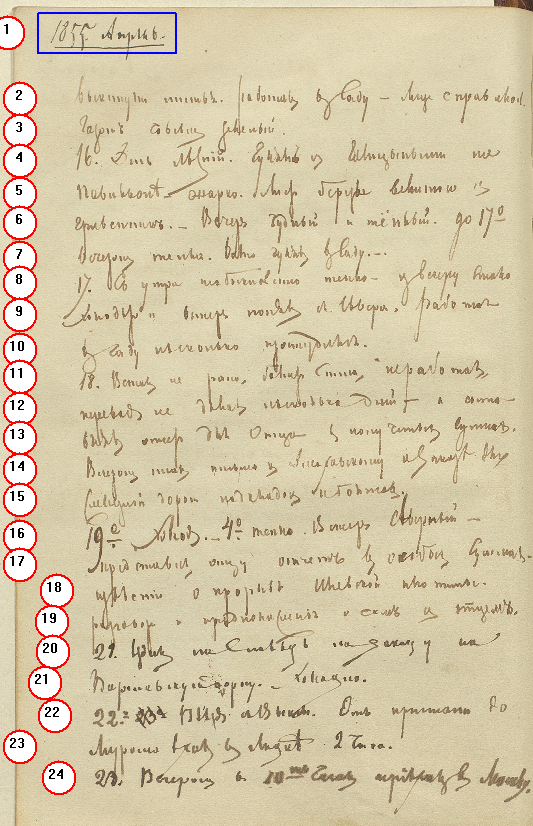
\includegraphics[width=\textwidth]{images/нарезка_на_строки_1.png}
	\end{minipage}
	%\hfill
	\begin{minipage}{0.49\textwidth}
		\centering
		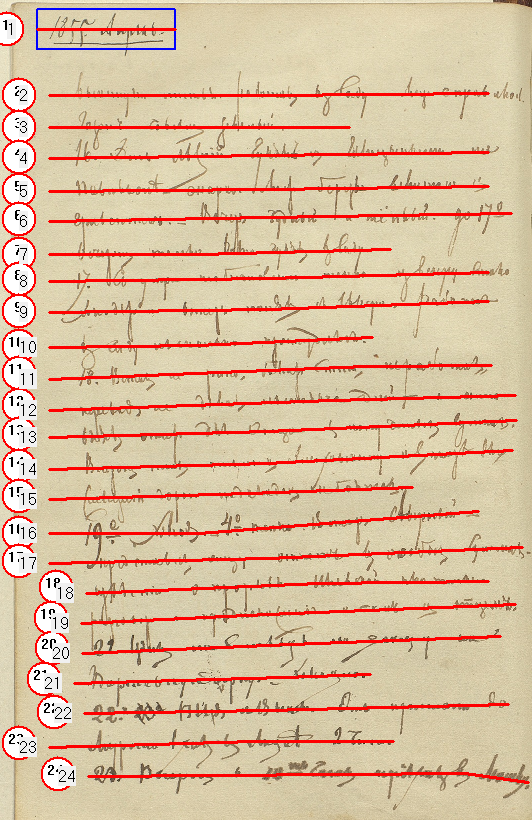
\includegraphics[width=\textwidth]{images/нарезка_на_строки_2.png}
	\end{minipage}
	\caption{Исходное изображение страницы, поданное в программу (слева) и изображение с выделенными базовыми линиями строк (справа)}
	\label{fig:line_detection_1_2}
\end{figure}

\subsubsection{Пример нормализации строк}

После выделения линий строк выполняется нормализация, в ходе которой строки выпрямляются для корректной подачи в модель. На рисунке \ref{fig:line_normalization} показана исходная строка и её нормализованный вид.

\begin{figure}[H]
	\centering
	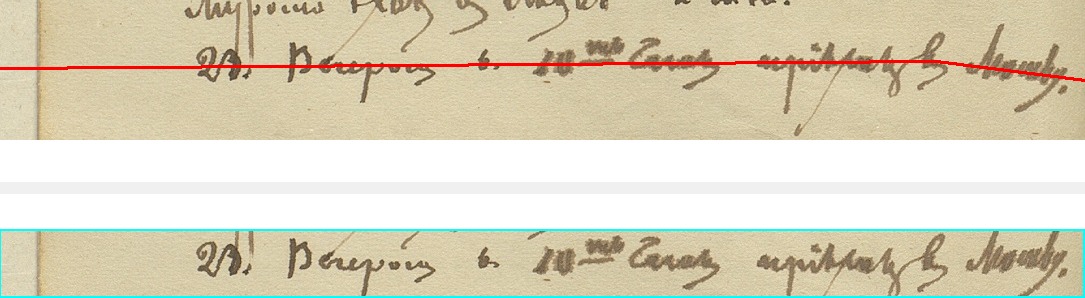
\includegraphics[width=0.99\textwidth]{images/нарезка_на_строки_3.png}
	\caption{Нормализация строки: исходная и выпрямленная строка}
	\label{fig:line_normalization}
\end{figure}


\section{Эксперименты}

\subsection{Эксперимент 1: Обучение на исходных RGB строках}

\textbf{Цель эксперимента}. В первом эксперименте проверялась возможность обучения строчной модели Vertical Attention Network (VAN) на строках, полученных из дневников А. В. Сухово-Кобылина. Гипотеза заключается в том, что строчная модель может достичь приемлемых показателей точности даже при ограниченном объёме данных, если использовать предварительное обучение на других датасетах.

\textbf{Постановка эксперимента}. Модель обучалась на 1505 строках (тренировочная часть), с валидацией на 119 строках и тестированием на 74 строках. Для инициализации весов кодировщика использовались веса, полученные при обучении на датасете IAM, а декодировщик обучался с нуля, поскольку алфавит отличается. Применялись аугментации, предложенные в статье о VAN \cite{VAN}. Модель обучалась 1 день на видеокарте NVIDIA A100 80GB, что составило 7802 эпохи.

\textbf{Графики метрик}. В ходе обучения отслеживались метрики CER и CTC-loss на тренировочной и валидационной выборках. Графики, показывающие динамику изменения метрик в зависимости от эпохи обучения, изображены на рис. \ref{fig:metrics_train_val}.

\begin{figure}[h!]
	\centering
	\begin{minipage}{0.49\textwidth}
		\centering
		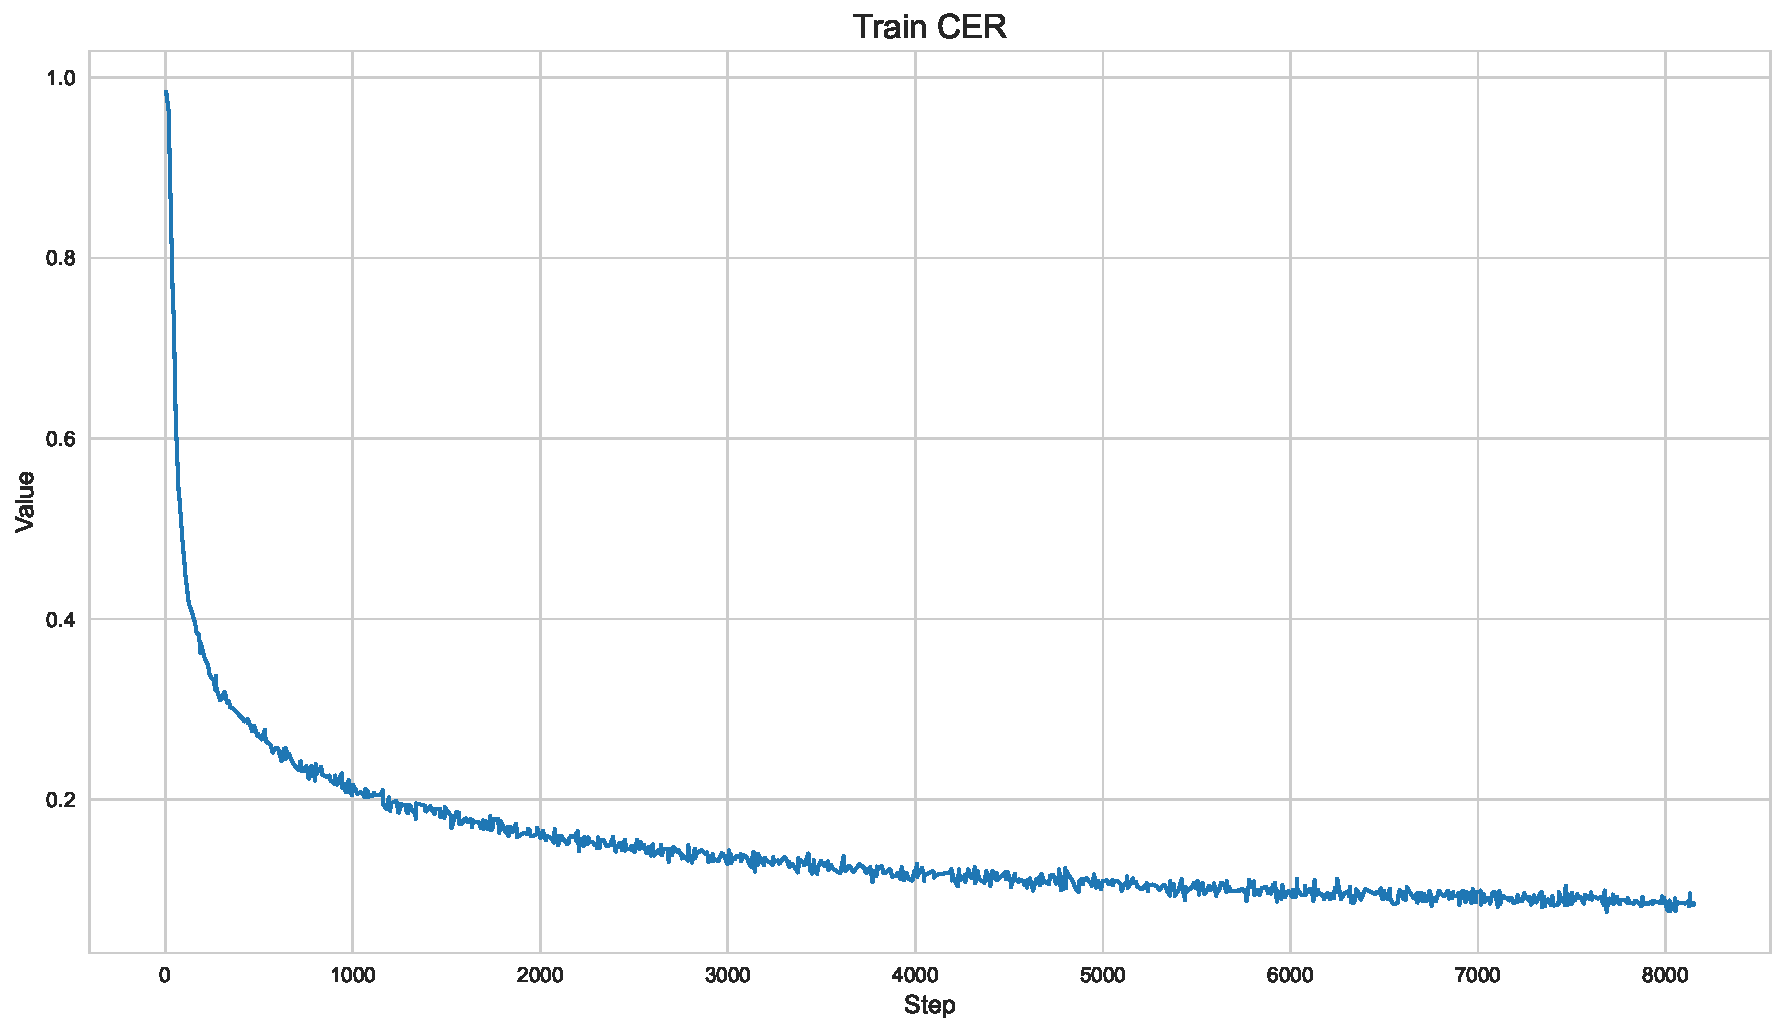
\includegraphics[width=\textwidth]{images/train_cer.pdf}
	\end{minipage}
	\begin{minipage}{0.49\textwidth}
		\centering
		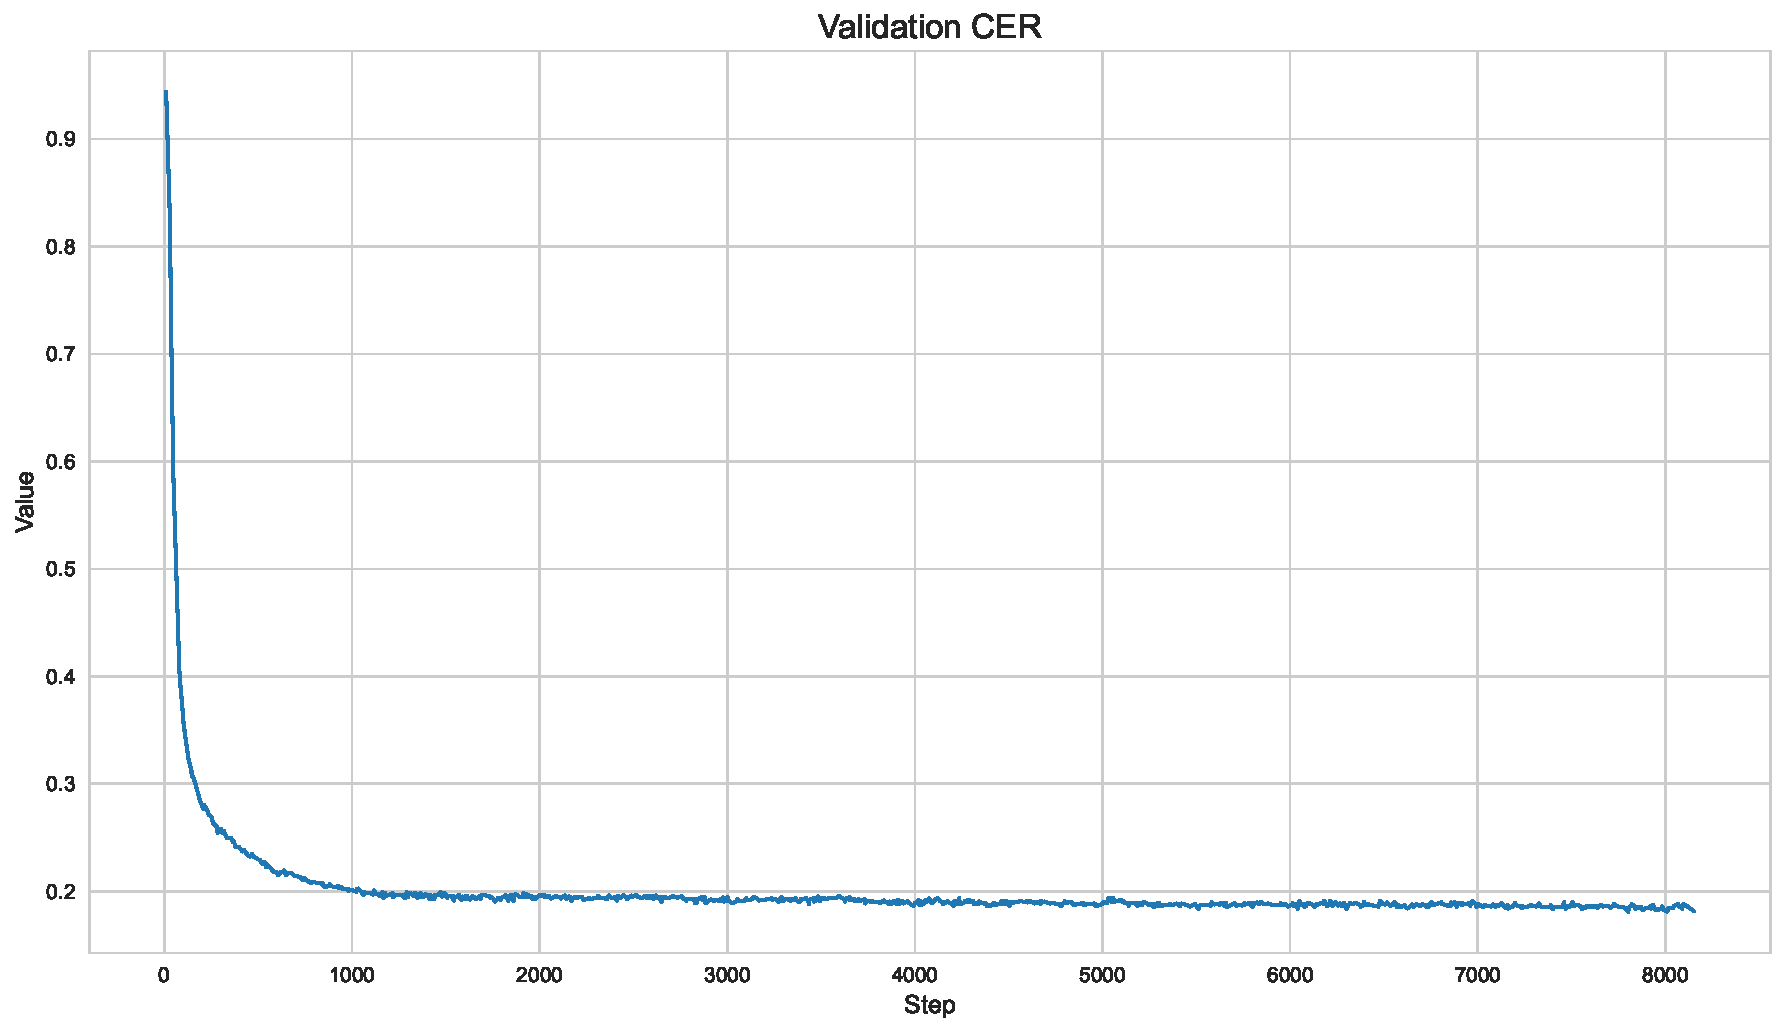
\includegraphics[width=\textwidth]{images/valid_cer.pdf}
	\end{minipage}
	\begin{minipage}{0.49\textwidth}
		\centering
		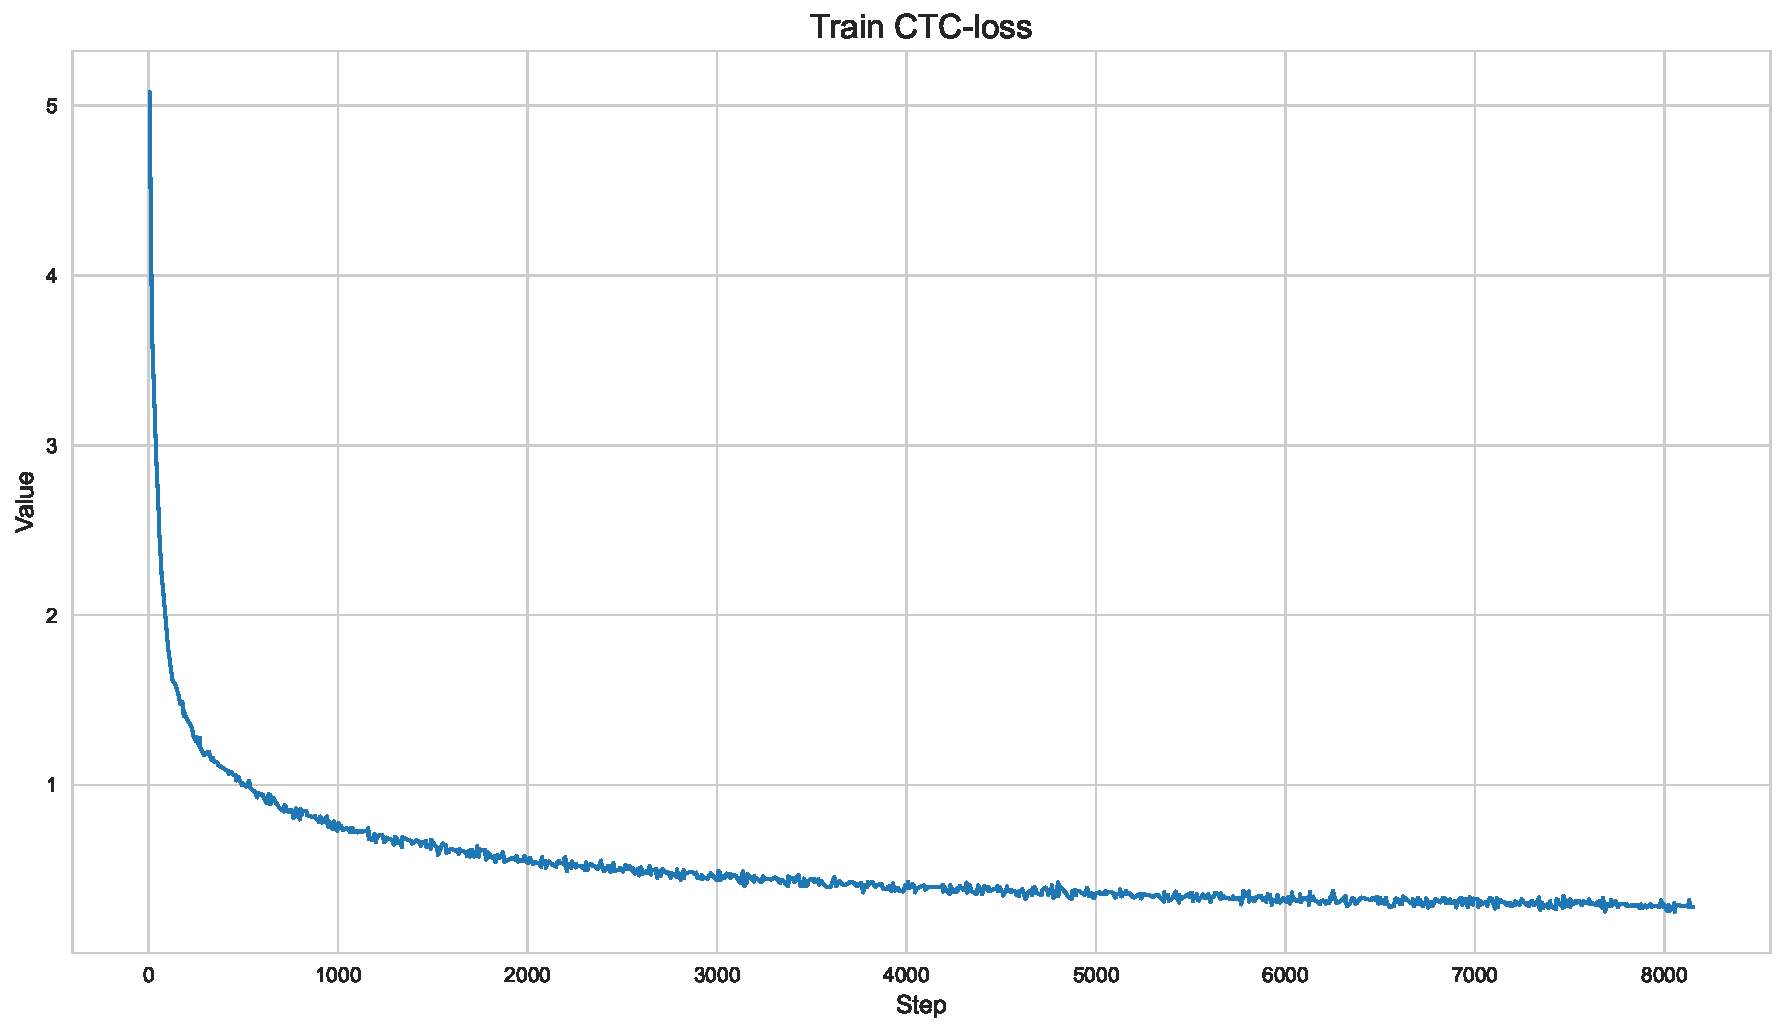
\includegraphics[width=\textwidth]{images/train_loss.pdf}
	\end{minipage}
	\begin{minipage}{0.49\textwidth}
		\centering
		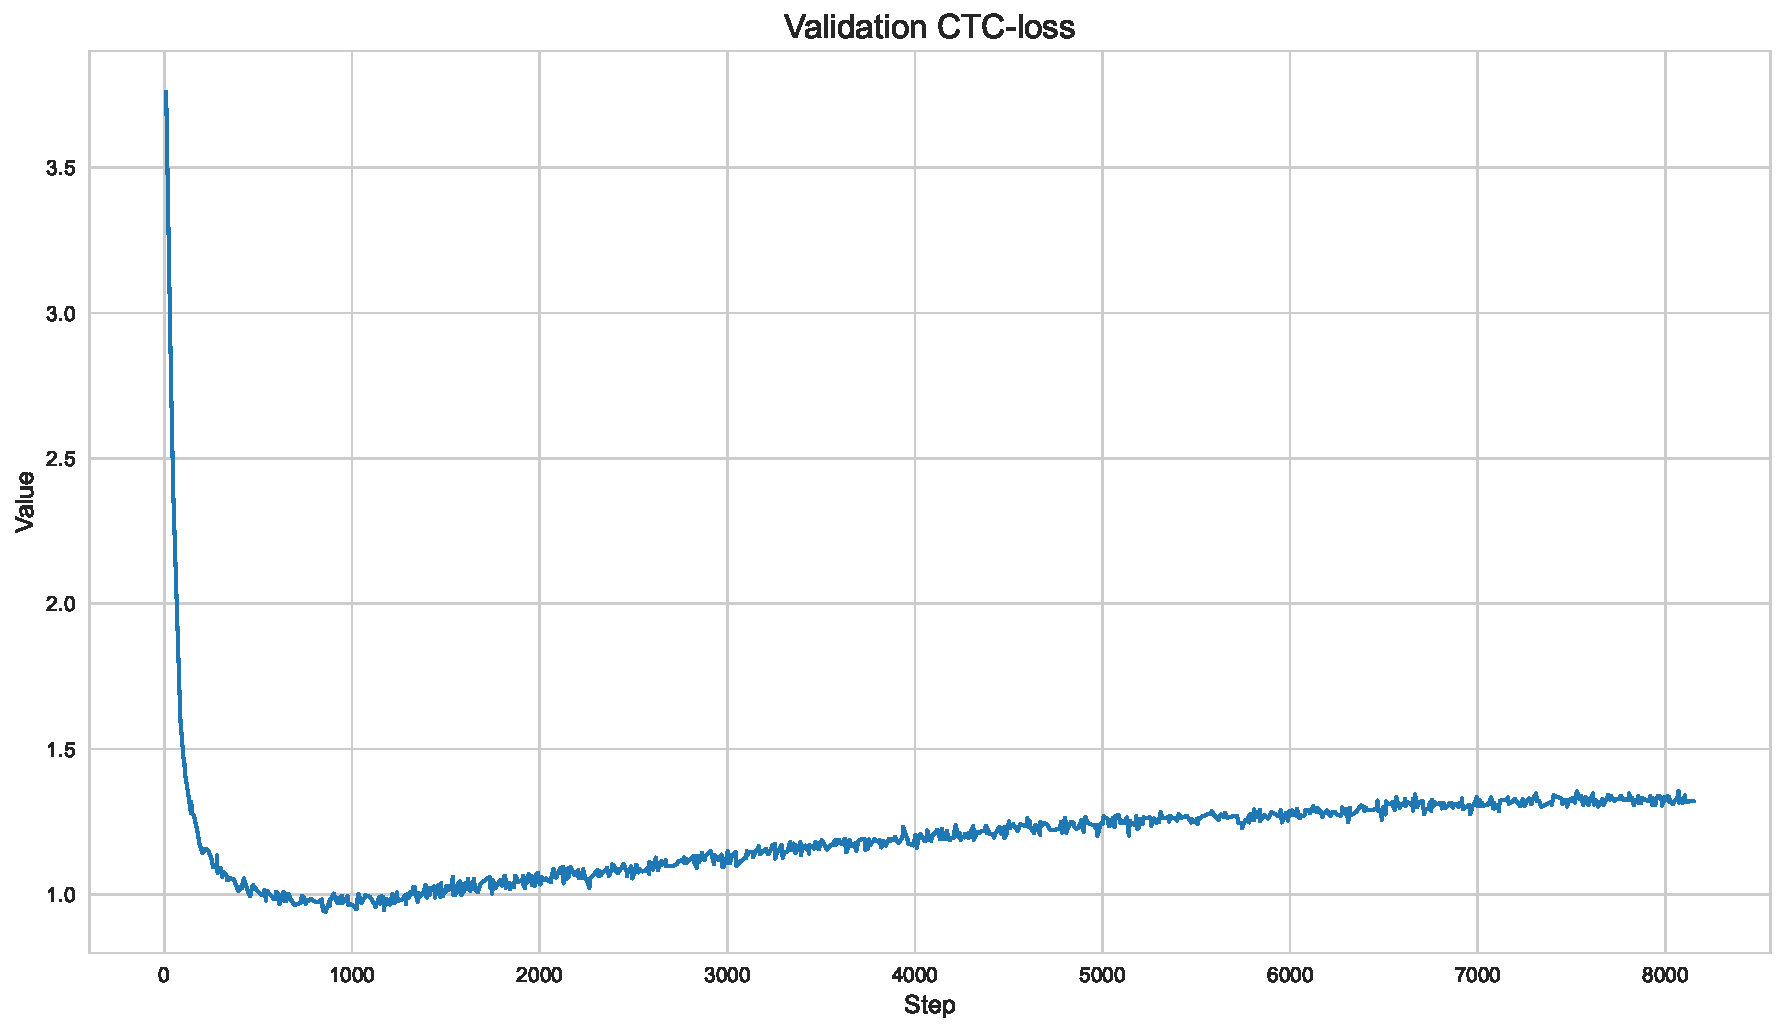
\includegraphics[width=\textwidth]{images/valid_loss.pdf}
	\end{minipage}
	
	\caption{CER (наверху) и CTC-loss (внизу) на тренировочной (слева) и валидационной выборке (справа)}
	
	\label{fig:metrics_train_val}
\end{figure}


\textbf{Результаты эксперимента}. Ниже приведены метрики CER и WER для тренировочной, валидационной и тестовой выборок:

\begin{table}[H]
	\centering
	\begin{tabular}{|c|c|c|}
		\hline
		& \texttt{CER} (\%) & \texttt{WER} (\%) \\
		\hline
		Тренировочная выборка & 0.37 & 1.03 \\
		\hline
		Валидационная выборка & 18.08 & 53.82 \\
		\hline
		Тестовая выборка & 19.03 & 52.44 \\
		\hline
	\end{tabular}
	\caption{Результаты на исходных данных}
	\label{tab:results_rgb}
\end{table}

\textbf{Примеры предсказаний}. На рис. \ref{fig:cv_examples} приведены примеры строк из тестовой выборки с расшифровкой, полученной моделью.

\begin{figure}[h!]
	\centering
	\begin{minipage}{0.99\textwidth}
		\centering
		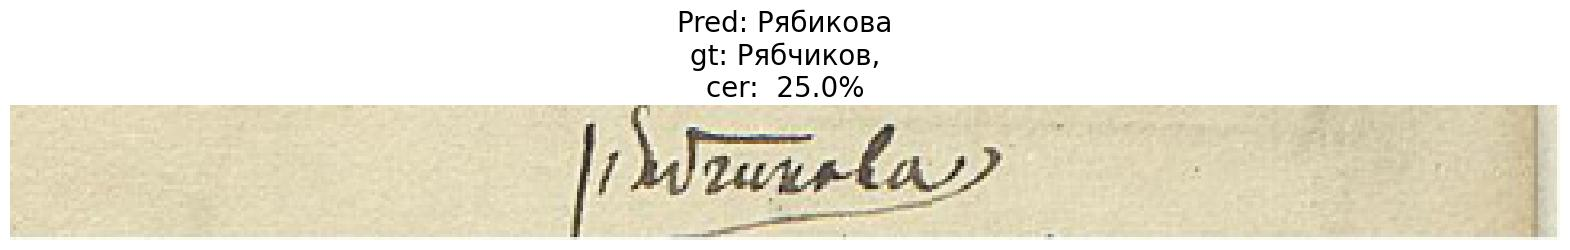
\includegraphics[width=\textwidth]{images/pred_1.jpg}
	\end{minipage}
	\begin{minipage}{0.99\textwidth}
		\centering
		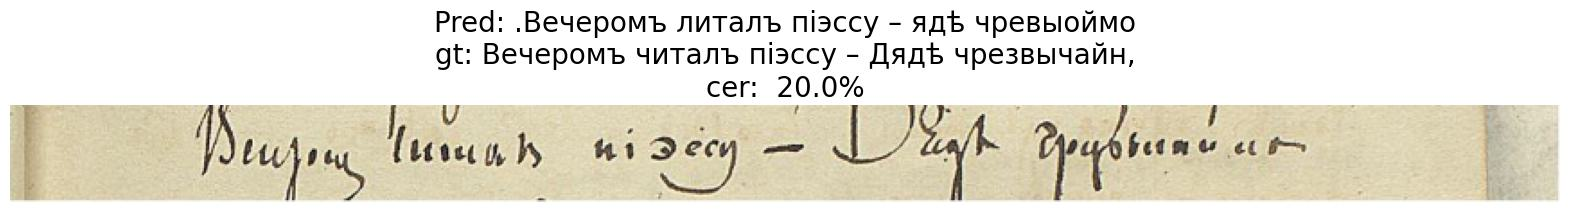
\includegraphics[width=\textwidth]{images/pred_2.jpg}
	\end{minipage}
	\begin{minipage}{0.99\textwidth}
		\centering
		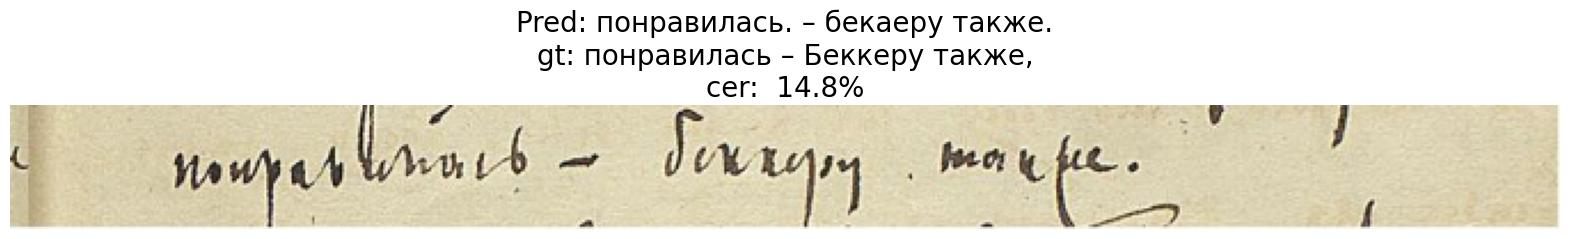
\includegraphics[width=\textwidth]{images/pred_3.jpg}
	\end{minipage}
	\begin{minipage}{0.99\textwidth}
		\centering
		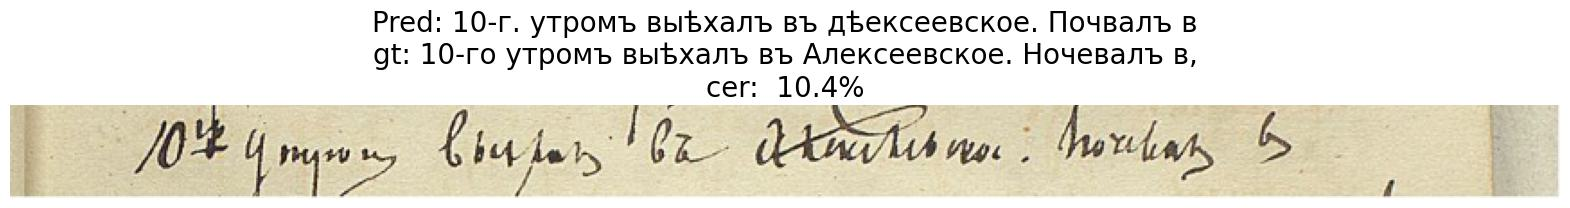
\includegraphics[width=\textwidth]{images/pred_4.jpg}
	\end{minipage}
	\begin{minipage}{0.99\textwidth}
		\centering
		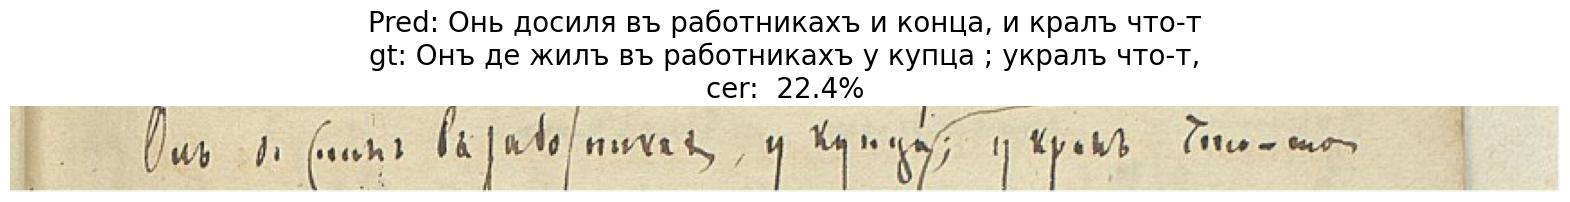
\includegraphics[width=\textwidth]{images/pred_5.jpg}
	\end{minipage}
	
	\caption{Примеры работы модели на тестовых данных: Pred -- предсказание, gt -- истинная разметка от экспертов}
	\label{fig:cv_examples}
\end{figure}

Модель допускает ошибки, однако многие слова, несмотря на ошибки, остаются понятными. Эти ошибки можно исправлять с помощью языковых моделей, например, ChatGPT.

\subsection{Эксперимент 2: Бинаризация строк и удаление свисающих элементов}

\textbf{Цель эксперимента}. Проверка гипотезы о том, что бинаризация строк и удаление свисающих элементов букв от других строк может улучшить качество распознавания.

\textbf{Постановка эксперимента}. Строки были бинаризованы: текст становился черным, фон — белым. Также были удалены свисающие элементы букв других строк. Для этого находились и удалялись небольшие по площади связные компоненты пикселей, примыкающие к границе прямоугольника текущей строки.

\textbf{Пример бинаризации}. На рис. \ref{fig:binarize_example} показаны исходная строка и её бинаризованный вид.

\begin{figure}[h!]
	\centering
	\begin{minipage}{0.99\textwidth}
		\centering
		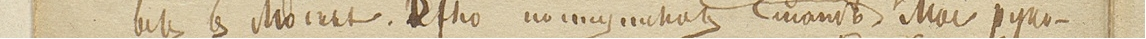
\includegraphics[width=\textwidth]{images/line_original.jpg}
	\end{minipage}
	\begin{minipage}{0.99\textwidth}
		\centering
		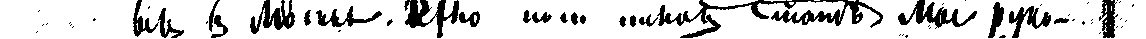
\includegraphics[width=\textwidth]{images/line_binarize.jpg}
	\end{minipage}
	
	\caption{Исходная строка и бинаризованная с убранными свисающими элементами}
	\label{fig:binarize_example}
\end{figure}

\textbf{Результаты эксперимента}. Результаты по метрикам для этого эксперимента оказались хуже по сравнению с исходными RGB-строками:

\begin{table}[H]
	\centering
	\begin{tabular}{|c|c|c|}
		\hline
		& \texttt{CER} (\%) & \texttt{WER} (\%) \\
		\hline
		Тренировочная выборка & 3.56 & 12.12 \\
		\hline
		Валидационная выборка & 24.33 & 65.12 \\
		\hline
		Тестовая выборка & 25.20 & 66.77 \\
		\hline
	\end{tabular}
	\caption{Результаты на бинаризованных данных с удаленными свисающими элементами}
	\label{tab:results_bin}
\end{table}

Модель обучалась всего 3588 эпох, так как после этого метрики на валидационной выборке вышли на плато. Предположительно, ухудшение качества связано с потерей информации во время бинаризации и неидеальным удалением свисающих элементов букв других строк.

\subsection{Эксперимент 3: Исправление ошибок с помощью ChatGPT}

\textbf{Цель эксперимента}. Проверить, может ли языковая модель ChatGPT улучшить расшифровку текста, предложенную моделью VAN.

\textbf{Постановка эксперимента}. Для исправления ошибок была использована модель ChatGPT-4o. Исправление выполнялось на уровне строк, так как исправление всей страницы может приводить к изменению количества строк, что нежелательно. Использовался подход few-shot learning, где в системном промпте содержались примеры из валидационной выборки.

Пример системного промпта:
\begin{quote}
	Твоя задача - корректировать входной текст, исправляя в нем ошибки.
	
	Это текст, распознанный моделью компьютерного зрения с рукописей. Рукописи написаны на русском языке 19 века (также иногда присутствуют другие языки).
	
	Цель - получить максимально близкий к рукописи вариант расшифровки.
	
	Модель допускает много ошибок в распознавании символов.
	
	Исправляй только самые явные и понятные места. Если фрагмент текста сложно разобрать, то сохраняй его в том же виде, в котором и получил.
	
	Сохраняй имена собственные и числительные как есть. Сохраняй исходную последовательность слов. \\
	
	Примеры: \\
	въ1 часовъ пріѣхалъ въ Камугу. Дядь притялъ меноя -> Въ 11 часовъ пріѣхалъ въ Калугу. Дядя принялъ меня \\
	Лучше. Смотрѣли иланъ моего завода – онъ далъ ое -> лучше. Смотрѣли планы моего Завода – онъ далъ мнѣ \\
	<Остальные примеры из валидационной выборки...> \\
\end{quote}

\textbf{Результаты эксперимента}. Первоначально строки исправлялись независимо, без учёта контекста предыдущих строк, то есть не учитывалась история исправления, и для каждой тестовой строки ассистент начинал сначала, используя только системный промпт. Этот подход дал следующие результаты на тестовой выборке: \textbf{CER = 18.86\%}, \textbf{WER = 44.31\%}. Таким образом, ошибка CER снизилась на 0.17\%, WER -- на 8.13\% по сравнению с первым экспериментом.

Далее был использован подход с сохранением истории предыдущих исправлений, так как в таком случае модель должна лучше понимать смысл текста, т.е. в при исправлении текущей строки в истории сохранялись сообщения пользователя и ответы ассистента с исправленными предыдущими строками. Такой подход улучшил результаты на тестовой выборке: \textbf{CER = 17.98\%}, \textbf{WER = 41.32\%}, т.е. ChatGPT уменьшил CER CV модели на 1.05\%, WER -- на 11.11\%.

\textbf{Примеры исправлений}. На рис. \ref{fig:gpt_example} показаны примеры строк, исправленных ChatGPT.

\begin{figure}[H]
	\centering
	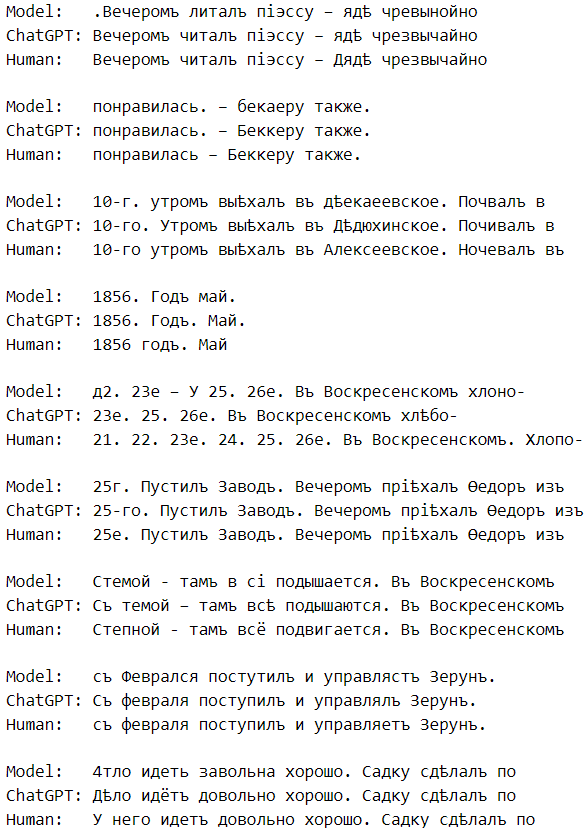
\includegraphics[width=0.61\textwidth]{images/gpt_example.png}
	\caption{Примеры исправленных строк: Model — результат CV модели, ChatGPT — результат исправления, Human — правильная разметка от экспертов-лингивистов.}
	\label{fig:gpt_example}
\end{figure}

Таким образом, использование ChatGPT позволило значительно снизить ошибки модели компьютерного зрения, особенно при учёте контекста предыдущих строк.


\section{Заключение}

В данной работе была представлена модель Vertical Attention Network (VAN), адаптированная для распознавания рукописных архивов А. В. Сухово-Кобылина. На основе предложенного метода были проведены эксперименты по обучению модели на нарезанных строках дневников, что позволило достичь метрик CER = 19.03\% и WER = 52.44\% на тестовой выборке. Было также исследовано влияние бинаризации строк и удаления свисающих элементов букв от других строк, что привело к ухудшению метрик. Однако использование ChatGPT в качестве языковой модели для пост-обработки позволило снизить ошибки модели до CER = 17.98\% и WER = 41.32\%.

Дальнейшие исследования будут направлены на улучшение процесса нормализации строк, а также на интеграцию других языковых моделей для исправления ошибок в тексте. Дополнительно планируется экспериментировать с различными архитектурами моделей для повышения точности распознавания и снизить зависимость модели от объема тренировочных данных.





\begin{thebibliography}{00}
	\bibitem{peter_dataset}
	Mark Potanin, Denis Dimitrov, Alex Shonenkov, Vladimir Bataev, Denis Karachev, Maxim Novopoltsev -- Digital Peter: Dataset, Competition and Handwriting Recognition Methods, arXiv:2103.09354 [cs.CV]
	
	\bibitem{SPAN}
	Denis Coquenet, Clement Chatelain, Thierry Paquet -- SPAN: a Simple Predict \& Align Network for Handwritten Paragraph Recognition, ICDAR 2021
	
	\bibitem{TrOCR}
	Minghao Li, Tengchao Lv, Jingye Chen, Lei Cui, Yijuan Lu, Dinei Florencio, Cha Zhang, Zhoujun Li, Furu Wei -- TrOCR: Transformer-based Optical Character Recognition with Pre-trained Models, CoRR 2022
	
	\bibitem{OrigamiNet}
	Mohamed Yousef, Tom E. Bishop -- OrigamiNet: Weakly-Supervised, Segmentation-Free, One-Step, Full Page Text Recognition by Learning to Unfold, CVPR 2020
	
	\bibitem{VAN}
	Denis Coquenet, Clement Chatelain, Thierry Paquet -- End-to-end Handwritten Paragraph Text Recognition Using a Vertical Attention Network, ICPR 2020
	
	\bibitem{IAM}
	Marti U.-V., Bunke H. -- The IAM-database: an English sentence database for offline handwriting recognition, IJDAR, 2002.
	
	\bibitem{CRNN}
	Shi B., Bai X., Yao, C. -- An End-to-End Trainable Neural Network for Image-Based Sequence Recognition and Its Application to Scene Text Recognition, TPAMI, 2017.
	
	\bibitem{CTC}
	Graves A., Fernandez S., Gomez F., Schmidhuber J. -- Connectionist Temporal Classification: Labelling Unsegmented Sequence Data with Recurrent Neural Networks, ICML 2006.
	
	\bibitem{yandex}
	Kopylov M., Artemov A., Stepanov S. -- Handwritten Text Recognition in Historical Documents: A Case Study on Russian Archives, arXiv:2103.09365 [cs.CV], 2022.
	
	\bibitem{transformer}
	Vaswani A., Shazeer N., Parmar N., et al. -- Attention is All You Need, NeurIPS 2017.
	
	\bibitem{ViT}
	Dosovitskiy A., et al. -- An Image is Worth 16x16 Words: Transformers for Image Recognition at Scale, ICLR 2021.
	
	\bibitem{transformer_decoding}
	Raffel C., et al. -- Exploring the Limits of Transfer Learning with a Unified Text-to-Text Transformer, JMLR, 2020.
	
	\bibitem{attentionocr}
	Borisov E., et al. -- AttentionOCR: A Novel Neural Network Architecture for Handwriting Recognition in Historical Manuscripts, ICPR, 2020.
	
	\bibitem{historical_handwriting}
	Puigcerver J. -- Are Multidimensional Recurrent Layers Really Necessary for Handwritten Text Recognition?, ICFHR, 2017.
	
	\bibitem{synthetic}
	Bartz C., et al. -- See, Read and Understand: End-to-End Neural Model for Handwritten Text Recognition, CVPR, 2017.
	
	\bibitem{handwriting_models}
	Shi B., et al. -- Handwritten Text Recognition: A Comprehensive Survey, TPAMI, 2018.
	
	\bibitem{DeepRec}
	Litman R., et al. -- DeepRec: A Deep Learning Approach for Offline Handwritten Text Recognition, ICASSP 2018.
	
	\bibitem{stepochkin}
	Stepochkin D. V. -- Methods of Handwriting Recognition for Russian Historical Archives, Moscow State University, 2024.
\end{thebibliography}



	
	
\end{document}